\documentclass[12pt, oneside]{article}
\usepackage[letterpaper, margin=1in, headsep=0.5in]{geometry}
\usepackage[english]{babel}
\usepackage[utf8]{inputenc}
\usepackage{amsmath}
\usepackage{amsfonts}
\usepackage{amssymb}
\usepackage{tikz}
\usetikzlibrary{quotes, angles}
\usepackage{graphicx}
%\usepackage{pgfplots}
%\pgfplotsset{width=10cm,compat=1.9}
%\usepgfplotslibrary{statistics}
%\usepackage{pgfplotstable}
%\usepackage{tkz-fct}
%\usepackage{venndiagram}

\usepackage{fancyhdr}
\pagestyle{fancy}
\fancyhf{}
\rhead{\thepage \\Name: \hspace{1.5in}.\\}
\lhead{BECA / Dr. Huson / 10th Grade Geometry\\* 26 October 2018}

\renewcommand{\headrulewidth}{0pt}

\begin{document}
\subsubsection*{Homework: Construct an altitude, distance application}
Use only a compass and straightedge for these classical constructions.
  \begin{enumerate}

  \item Construct a perpendicular to $\overline{AB}$ though $C$.\\
    %\hspace{1cm} Given the line  $l$ and point $P$.
    \vspace{2cm}
    \begin{center}
    \begin{tikzpicture}
      \draw [<->, thick] (0,0)--(11,0)--(6,4)--cycle;
      \draw [fill] (0,0) circle [radius=0.05] node[left]{$A$};
      \draw [fill] (11,0) circle [radius=0.05] node[right]{$B$};
      \draw [fill] (6,4) circle [radius=0.05] node[above right]{$C$};
    \end{tikzpicture}
  \end{center} \vspace{5cm}

  \item Given the conditional statement, ``If the corresponding angles of a transversal are congruent, then the two lines are parallel."
    \begin{enumerate}
      \item Write down the hypothesis. \vspace{1.5cm}
      \item Write down the converse of the statement. \vspace{2cm}
      \item Write down the contrapositive of the statement. \vspace{1.5cm}
    \end{enumerate}

\newpage
\item Given the quadrilateral $RSTU$ with $R(1,3)$, $S(4,7)$, $T(4,2)$, and $U(1,-2)$.
\begin{enumerate}
  \item Plot and label $RSTU$ on the grid.
  \item Using the distance formula or otherwise, calculate $RS$, $ST$, $TU$, and $RU$.
  \item Definition: If a quadrilateral has four congruent sides, then it is a rhombus.\\[0.5cm]
  Prove that $RSTU$ is a rhombus.
\end{enumerate}

\begin{center} %4 quadrant regents grid w T-Chart
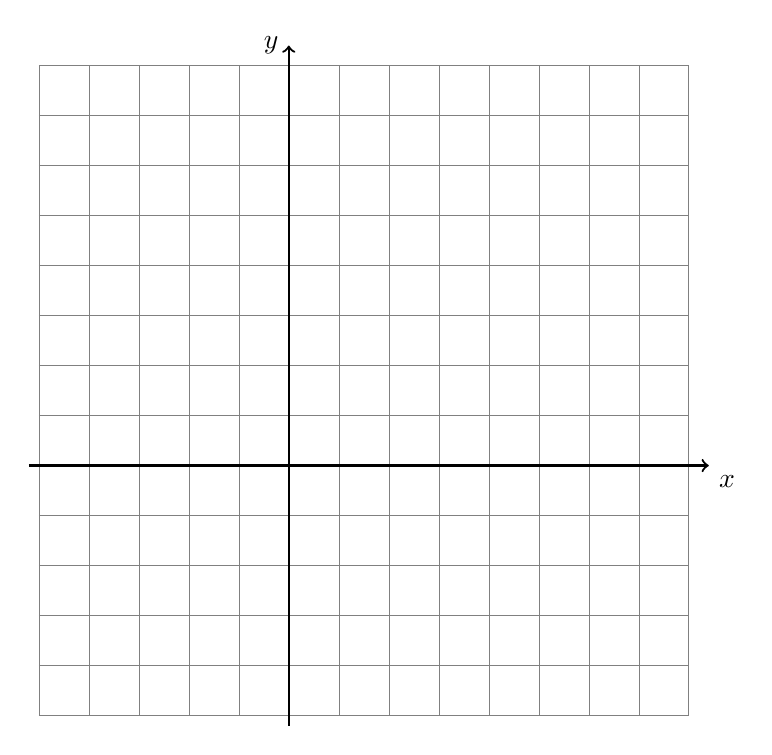
\begin{tikzpicture}[scale=.635]
  \draw [help lines] (-5,-5) grid (8,8);
  \draw [thick, ->] (-5.2,0) -- (8.4,0) node [below right] {$x$};
  \draw [thick, ->] (0,-5.2)--(0,8.4) node [left] {$y$};
\end{tikzpicture}
\end{center}


\end{enumerate}
\end{document}
